%%
%% This is file `sample-sigconf.tex',
%% generated with the docstrip utility.
%%
%% The original source files were:
%%
%% samples.dtx  (with options: `sigconf')
%%
%% IMPORTANT NOTICE:
%%
%% For the copyright see the source file.
%%
%% Any modified versions of this file must be renamed
%% with new filenames distinct from sample-sigconf.tex.
%%
%% For distribution of the original source see the terms
%% for copying and modification in the file samples.dtx.
%%
%% This generated file may be distributed as long as the
%% original source files, as listed above, are part of the
%% same distribution. (The sources need not necessarily be
%% in the same archive or directory.)
%%
%% The first command in your LaTeX source must be the \documentclass command.
\documentclass[sigconf, review]{acmart}

%%
%% \BibTeX command to typeset BibTeX logo in the docs
\AtBeginDocument{%
  \providecommand\BibTeX{{%
    \normalfont B\kern-0.5em{\scshape i\kern-0.25em b}\kern-0.8em\TeX}}}

%% Rights management information.  This information is sent to you
%% when you complete the rights form.  These commands have SAMPLE
%% values in them; it is your responsibility as an author to replace
%% the commands and values with those provided to you when you
%% complete the rights form.
\setcopyright{acmcopyright}
\copyrightyear{2020}
\acmYear{2020}
\acmDOI{10.1145/1122445.1122456} %% TODO

%% These commands are for a PROCEEDINGS abstract or paper.
\acmConference[ICSE 2020]{International Conference on Software Engineering}{May 23--29, 2020}{Seoul, South Korea} 
\acmBooktitle{ICSE '20: Internation conference on Software Engineering, May 23--29, 2020, Seoul, South Korea}
\acmPrice{15.00} % % TODO
\acmISBN{978-1-4503-9999-9/18/06} % % TODO


%%
%% Submission ID.
%% Use this when submitting an article to a sponsored event. You'll
%% receive a unique submission ID from the organizers
%% of the event, and this ID should be used as the parameter to this command.
%%\acmSubmissionID{123-A56-BU3}

%%
%% The majority of ACM publications use numbered citations and
%% references.  The command \citestyle{authoryear} switches to the
%% "author year" style.
%%
%% If you are preparing content for an event
%% sponsored by ACM SIGGRAPH, you must use the "author year" style of
%% citations and references.
%% Uncommenting
%% the next command will enable that style.
%%\citestyle{acmauthoryear}

%%
%% end of the preamble, start of the body of the document source.
\begin{document}

%%
%% The "title" command has an optional parameter,
%% allowing the author to define a "short title" to be used in page headers.
\title{Employing Students for the Creation of Institutional Software}

%%
%% The "author" command and its associated commands are used to define
%% the authors and their affiliations.
%% Of note is the shared affiliation of the first two authors, and the
%% "authornote" and "authornotemark" commands
%% used to denote shared contribution to the research.
\author{Bria Williams}
\affiliation{%
  \institution{Berea College}
  \streetaddress{101 Chestnut St}
  \city{Berea}
  \state{Kentucky}
  \postcode{40403}
  \country{USA}}
\email{williamsbri@berea.edu}


\author{Katelyn Adams}
\affiliation{%
  \institution{Berea College}
  \streetaddress{101 Chestnut St}
  \city{Berea}
  \state{Kentucky}
  \postcode{40403}
  \country{USA}}
\email{adamska@berea.edu}

\author{Scott Heggen}
\affiliation{%
  \institution{Berea College}
  \streetaddress{101 Chestnut St}
  \city{Berea}
  \state{Kentucky}
  \postcode{40403}
  \country{USA}}
\email{heggens@berea.edu}

%%
%% By default, the full list of authors will be used in the page
%% headers. Often, this list is too long, and will overlap
%% other information printed in the page headers. This command allows
%% the author to define a more concise list
%% of authors' names for this purpose.
\renewcommand{\shortauthors}{Williams, Adams, and Heggen}

%%
%% The abstract is a short summary of the work to be presented in the
%% article.
\begin{abstract}
 Higher educational institutions, like most all large businesses, need to purchase third-party software to manage their daily operations. Because of limited budgets, the costs to purchase some needed software is prohibitive, resulting in the purchase of less apt software, or none at all. These limitations lead to interfaces that are sometimes difficult to use, poorly developed, not fully-featured for the needs of the institution, or simply the wrong tool for the job. Worse yet, contracts lock institutions into this software for multiple years, putting a strain on the faculty, staff, and students who rely on the software. The tech support by these companies is not always easily accessible and costs the institution more money. As an alternative solution, a team of student developers led by a faculty and minimal staff support can create custom, institution-specific software that meets the college's unique needs while providing students with valuable work experience building their skills and preparing them for software engineering positions after graduation. This paper highlights the successes of a five-year experiment employing college students as software developers creating software for a higher education institution.

% 164 words
\end{abstract}

%%
%% The code below is generated by the tool at http://dl.acm.org/ccs.cfm.
%% Please copy and paste the code instead of the example below.
%%
\begin{CCSXML}
<ccs2012>
<concept>
<concept_id>10002951.10003227.10003233.10003597</concept_id>
<concept_desc>Information systems~Open source software</concept_desc>
<concept_significance>500</concept_significance>
</concept>
<concept>
<concept_id>10002951.10003227.10003228.10003442</concept_id>
<concept_desc>Information systems~Enterprise applications</concept_desc>
<concept_significance>300</concept_significance>
</concept>
<concept>
<concept_id>10002951.10003227.10003228.10003229</concept_id>
<concept_desc>Information systems~Intranets</concept_desc>
<concept_significance>100</concept_significance>
</concept>
<concept>
<concept_id>10010405.10010489.10010491</concept_id>
<concept_desc>Applied computing~Interactive learning environments</concept_desc>
<concept_significance>500</concept_significance>
</concept>
<concept>
<concept_id>10010405.10010489.10010492</concept_id>
<concept_desc>Applied computing~Collaborative learning</concept_desc>
<concept_significance>500</concept_significance>
</concept>
<concept>
<concept_id>10011007.10011006.10011066.10011070</concept_id>
<concept_desc>Software and its engineering~Application specific development environments</concept_desc>
<concept_significance>300</concept_significance>
</concept>
</ccs2012>
\end{CCSXML}

\ccsdesc[500]{Information systems~Open source software}
\ccsdesc[300]{Information systems~Enterprise applications}
\ccsdesc[100]{Information systems~Intranets}
\ccsdesc[500]{Applied computing~Interactive learning environments}
\ccsdesc[500]{Applied computing~Collaborative learning}
\ccsdesc[300]{Software and its engineering~Application specific development environments}

%%
%% Keywords. The author(s) should pick words that accurately describe
%% the work being presented. Separate the keywords with commas.
\keywords{Software Engineering, Collaborative Learning, Informal Learning Environments, CS Education}

%% A "teaser" image appears between the author and affiliation
%% information and the body of the document, and typically spans the
%% page.
% \begin{teaserfigure}
%   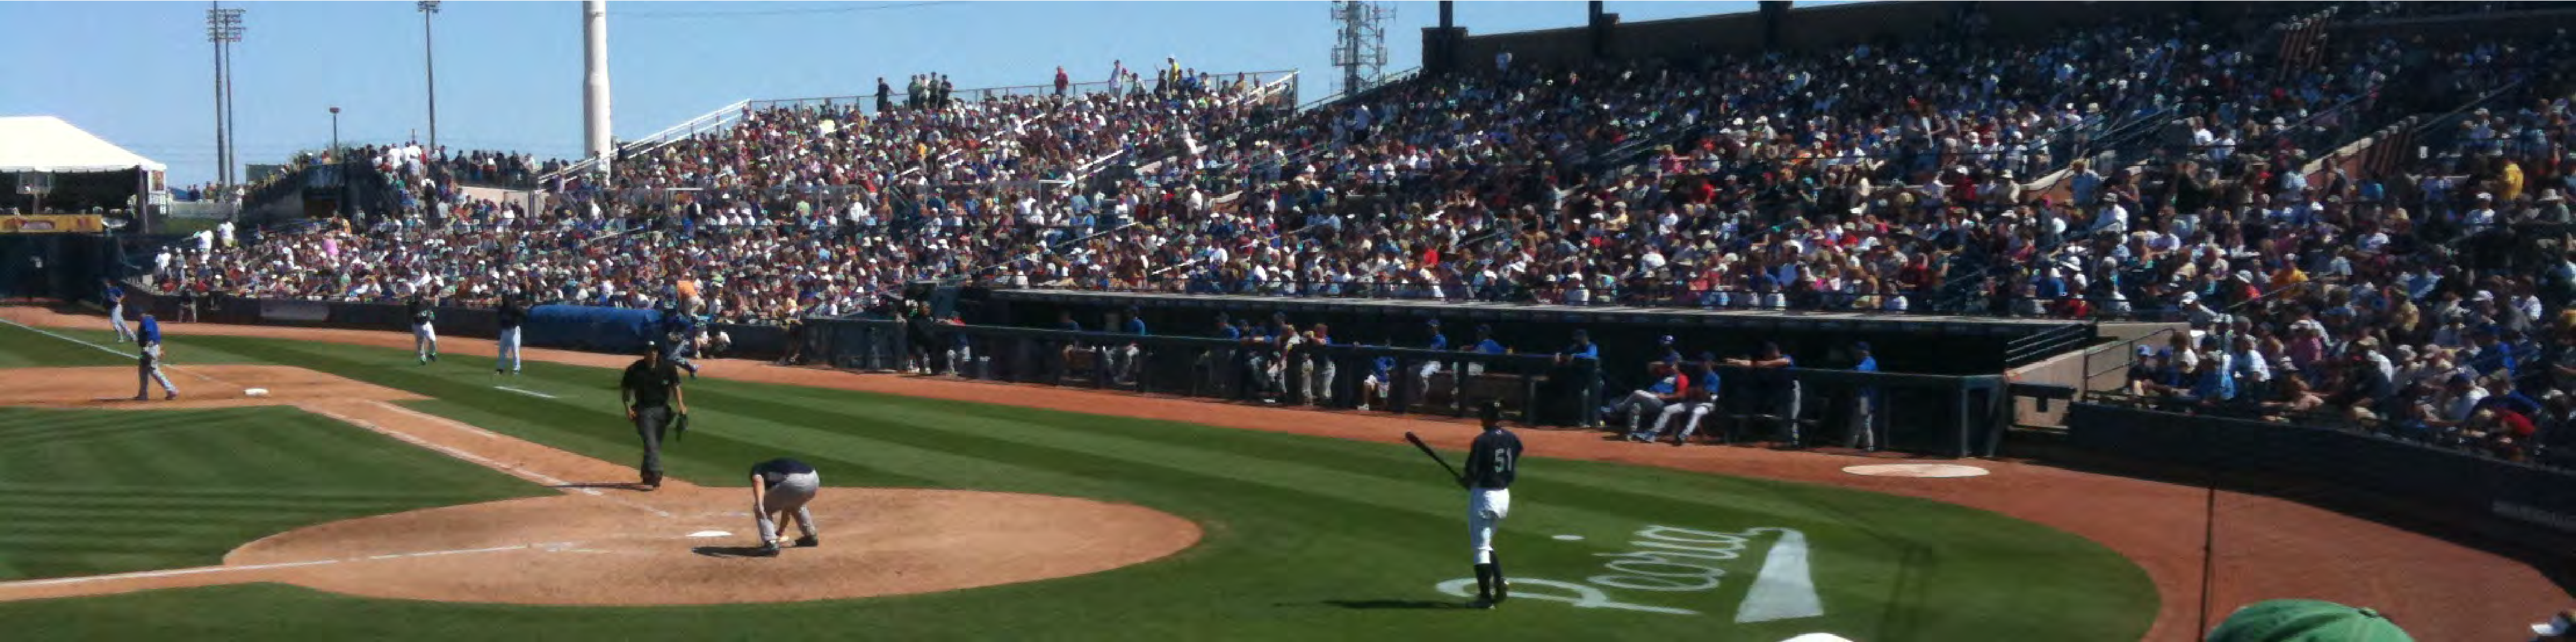
\includegraphics[width=\textwidth]{sampleteaser}
%   \caption{Seattle Mariners at Spring Training, 2010.}
%   \Description{Enjoying the baseball game from the third-base
%   seats. Ichiro Suzuki preparing to bat.}
%   \label{fig:teaser}
% \end{teaserfigure}

%%
%% This command processes the author and affiliation and title
%% information and builds the first part of the formatted document.
\maketitle

% Outline:
% Writing Software to Impact Higher-Education Institutions
%   Abstract: Evaluating the impact/success of software projects in higher-education institutions {Berea College}
%   Introduction
%   Development
%       Related Work/Research [Project Success Research]
%       Methods - [Evaluation of: software efficiency, impact on the customer, direct business and organizational                     success]
%       Results/Discussion
% Conclusion/Next Steps

\section{Introduction}

The growing complexity of higher education institutions means an increasing reliance on technology, in particular, software. Most institutions rely heavily on databases and management platforms, such as Banner \cite{BannerWebsite}, to manage the complexity. Similarly, learning management systems such as Moodle \cite{MoodleWebsite} and Blackboard \cite{BlackboardWebsite} improve the educational experience of students and faculty by facilitating and automating common tasks such as grading and distributing information to classes. Some of the software is open source (e.g., Moodle), which means the software itself is free, but the customization and support of the software costs the institution. Proprietary software typically has a combination of an initial purchase cost, a maintenance cost, and a multi-year contract. While the software can receive good support from the developers and institution-specific customization as-needed, the annual costs can creep into the thousands of dollars per application. According to a 2015 report about higher education spending, it is estimated that higher education institutions spend on average 4.2\% of their entire budget on information technology alone \cite{CDSBenchmarkReport}. 

%CUT - As technology advances, users' needs follow suit. Higher educational institutions are forced to adapt with the times, and their processes are making the transition from paper to digital. Many expensive software programs have been developed for these purposes and are on the market. 

%CUT - However, not all purchasable third-party software is suitable for a college's specific needs. An institution can spend upwards of around \$4,000 dollars [I did a simple google search of school administration costs but like..is there something we can cite for this? also i cant put a dollar sign..-kat] on software 

These applications are built to meet the general needs of managing higher education, such as course registration and scheduling, but do not handle the nuanced difference that exist at every institution. For example, some institutions operate on a typical semester calendar consisting of a Fall, Spring, and Summer term. Other institutions may operate on a quarterly calendar, or they may have other terms such as a January short-term, multiple summer terms, online courses without specific start and end dates, or not operate on a calendar system at all. These institution-specific modifications are supported by software developers through ``additional services'' they provide. In other words, they are going to cost the institution on top of the base cost of the software.

Worse yet, each institution is unique in its needs, and sometimes the software simply doesn't exist. For example, there are nine work colleges in the United States \cite{WCCMembers, Ecclesia}. A work college requires every student to be employed while attending, and student employment is considered a part of the institution's academic mission. Given there are only nine work colleges, there isn't a market for the creation of large-scale software to support work colleges. However, there is a lot of need for software to manage a work college, such as tracking student employment, time-sheets for clocking hours, reporting back to the federal government and other funding sources, and evaluating student and supervisor performance, to name a few. Again, custom software is expensive and adds to the cost of managing the institution. In the case of work colleges, which tend to be smaller institutions, this cost is particularly prohibitive. 

An institution could hire a permanent team of software engineers to craft a custom applications. This is rare, however, as most institutions do not have the expertise on campus to manage a software engineering team. Software engineers tend to be expensive to hire, and often move jobs frequently due to a vibrant market. 

However, an institution's unique needs can be met by a team of students crafting custom, institution-specific software. Instead of hiring an entire software engineering team, a faculty member or staff member can serve as a project manager to the team of students, guiding them in the development of software without dedicating their entire time to writing the code itself. 

%Through close communication with customers, the team can create simple, custom interfaces that save not only resources by rendering dated paper processes unnecessary, but time and money as these processes do not take as long and human error decreases. 

As an added benefit, the students gain valuable experience, preparing them for the software engineering industry after graduation. The students learn numerous technical skills \cite{hardskills}, such as specific programming and markup languages, software engineering principles, libraries, frameworks, web development, MVC, and more. Students also learn a number of valuable soft skills, such as critical thinking, leadership, project and time management, teamwork, and problem solving; skills deemed valuable for new graduates to have by employers \cite{lavy2013soft}. Similar studies 

By recruiting a team of student software developers, a college can not only avoid the high cost of software and get applications that are tailored specifically to meet their needs, but also provide students with valuable experience that better prepares them for the industry. 

This paper describes a program which blends the best parts of a software engineering course and an external experience like an internship. Through a work-study program, students are employed by the computer science department to develop software for a full year. Teams of students start in the summer, working approximately 400 hours under the supervision of a faculty member, where they are trained on the software engineering principles and apply them to in-progress projects or new ones. The projects are proposed by the campus community (a.k.a. the customer) and are then selected by the faculty member supervising the team. These projects are often tools requested by the customer to help them complete their daily work, and thus, the software becomes an integral part of the customer's job. Students intend to finish the beta version of the product by the end of summer and have customer demos and reflection on the team's performance. During the academic year, Fall and Spring terms, the students work an additional 300 or more hours, where they maintain the software; implementing new feature requests, fixing bugs,and performing prompt, free customer support. 

The remainder of this paper is organized as follows: the Related Work section describes research and programs related to undergraduate software engineering. Next,the methodology for implementing meaningful a year-long software development internship experience is proposed. Finally, we will observe and analyze the specific results of the Student Software Development Team's look into the effectiveness of our software.

%%[Diagram of software dev cycle]
%%[Diagram of fall spring vs summer]
% \section{Related Work}
[Kat asks that Scott help her with this section]

[CITE THIS https://www.nytimes.com/2014/08/28/nyregion/students-inventing-programs-to-streamline-their-colleges-data.html] 
In 2013, 19 students at Baruch College used a script to query for openings in crowded courses; they did so at such high frequencies that they nearly took down their institution's system. A student at Rutgers University grew frustrated at his inability to get into popular courses; he built a tool that queried the university's registration system and by the next semester, 8,000 people had used it. These encounters show the difficulty of retrieving necessary data from dated school information systems. 
[To be continued...]
\subsection{}

\subsubsection{Third layer of hell}

\cite{heggen2018hiring}
\section{Methods}
%%This section is due Sept 14th!!
%Needs paragraph formatting, content chunking, etc
A.   The Team

The Berea College Student Software Development Team (referenced henceforth as the SSDT) is comprised of six to ten undergraduate students of all levels who typically are majoring or minoring in Computer and Information Sciences, two staff members (one of whom is an alumni of the Computer Science program), and a Computer Science faculty member who serves as the Scrum Master. The SSDT work year-round improving, designing, developing, and managing software for the institution using Agile methodologies. The SSDT recieves requests from departments and offices at the college who are in need of improvements to their current software, a complete refactoring of their current software, or in some cases, are still using inefficient paper processes and have no software currently in use. Typically project requests are recieved via email or during a discussion of the customer's current status of their processes. It is also not unlikely for the Scrum Master to reach out to offices and departments throughout the institution and inquire about the existing software (or lack thereof).  When a software request is recieved, the team* reviews the components of each request and determine which software to prioritize for the year. The team decides which software request will be the main focus based on the which has the greatest need. This decision is based on the request's urgency, importance, value to the institution, and the effort it will take to implement. Urgency is determined by how soon the requestor needs the software, i.e. if the requestor's office is currently running so inefficiently on their current processes that it affects other offices on campus. Importance and value is considered based upon how largely the implementation will be used at the institution. Last, effort is evaluated by the time, number of student programmers it will take to bring the request to completion. All of these factors are weighed in order to select the request that requires the most immediate attention. After a request is determined* to need improvements in all of these areas, it is selected as the center of focus for the year. 



 Measuring Success
The objective of the study is to demonstrate the impact of software developed predominantly by undergraduate students has on higher educational institutions. To determine the impact that the student-developed software has had on the institution several factors of software success are identified and evaluated.  There exists much research on quantifying project success. For this study, the metrics for software success were defined using DeLone and McLean’s Model for Information Software Success. (CITATION NEEDED) This model consists of six measures of success which included the following: system quality, information quality, use, user satisfaction, individual impact, and organizational impact. These measures may be used to evaluate the software systems based on factors including but not limited to, code quality, appearance, usability, relevance, and cost reduction.  A survey comprised of questions that derive from each of these six components was constructed. There are seven software systems that are currently in production at the institution allowing for a multiple case study (CITATION NEEDED).

    Participants
Participants in this study included [INSERT NUMBER of PEOPLE HERE] Berea College faculty and staff. All participants in this study were volunteers and were administered a survey pertaining only to the software that they had interacted with. The survey was only sent to those who were the primary users and/or had administrative privileges to the software. This pool of faculty members was selected, as opposed to surveying all users, because these subjects were involved in the initial phase of the software development process, which is defining the software project’s scope and the needs of the customer. [CITATION?] Each survey began with an informed consent disclaimer that detailed the nature

The SSDT has eight systems that we handle. These include the Advancement Office, BCAC, BCSR, CAS, LSF, Ulmann, URCPP, and SKYZ. Each system has a specific functionality to aid our faculty and staff clientele perform their jobs. For example, CAS (Course Administration and Scheduling) helps the registrar, as well as faculty and staff, schedule terms, manage courses, programs, divisions, and much more.
We distributed our surveys and gave our clients two weeks to submit their responses. We barely got over 50 percent participation (9/17 survey responses were submitted)


%%should we have a paragraph for each system? Acronym breakdown, client, and system description??  Kat
Quantitative data (stats)
%I think we should include all possible responses for questions like "how important is it" to show what responses the clients were given to choose from
Of our 9 responses: %I started at column D in Data Analysis spreadsheet since the first three were not quantitative
How often do you use the software? daily use: 3, weekly use: 1, monthly use: 4, yearly use: 1.
Each time you use the  application, how long do you interact with it?: < 15 minutes: 1, 15-30 mins: 3, 30 mins - 1 hr: 4, 1 - 2 hrs: 1.
How much of your day-to-day responsibilities depend on your ability to use the  application? Important: 4, Essential: 5.
How much do you agree with each of the following statements?
[Using this application allows me to do my job better]: Strongly Disagree: 1, Neutral: 1,Agree: 1, Strongly Agree: 6.
[Using this application allows me to do my job faster]: Strongly Disagree: 1, Disagree: 1, Agree: 1, Strongly Agree: 6
[My level of competency with software is not relevant when using the software] Disagree: 1, Neutral: 4, Agree: 2 Strongly Agree: 2
%The next questions are system specific functionality/ease of use so we will have to represent that data in some other way...Since each system had different (sometimes 1, sometimes multiple, functionalites here (cas has a lot, BCSR has 1.)
%If system was gone, what would it cost client?
If the software were to be taken down entirely, what would it cost you in terms of:
Stress:
Time:
Errors:
Money:
%Comparison of system to other non SSDT software(moodle,banner, etc)
How would you estimate the value of the software compared to Berea College's following applications?
Banner:
MyBerea:
Degree Works:
Moodle:
Online Bookstore:
TRACY:
College email:
Password Management site:
Hutchins library site:

\section{RESULTS}
% MOVE This internship model has produced such favorable outcomes that it has been implemented consecutively for five years. Early on, the team took on every project that was pitched to the team, resulting in five applications in the first five years. However, by the third year, the team had to bear in mind the maintenance of existing systems in addition to creating new software. Adoption slowed, but did not stop...

\subsection{Study Design}
In order to demonstrate the impact of software developed predominantly by undergraduate students has on higher educational institutions, several factors of software success were identified and evaluated.  The metrics for software success were informed primarily by DeLone and McLean's Model for Information Software Success \cite{delone1992softwaresuccess}. Their model consists of six measures of success: system quality, information quality, use, user satisfaction, individual impact, and organizational impact. Additionally, the SSDT leveraged the Agile Manifesto \cite{agilemanifesto} as a guiding set of principles for developing software. A survey was developed and issued to the product owners of each of the eight applications built by the SSDT. Questions were derived from four of these six components from DeLone and McLean (system quality and information quality were excluded, since product owners are not always able to accurately judge these metrics), as well as principles from the Agile Manifesto. % TODO what metrics from AM and how were our PO's able to judge them?

\subsection{Participants}
Participants in this study included 14 institutional faculty and staff who all represented product owners, in that they were administrators in the systems and had the largest amount of interactions with the software. Ten out of the fourteen clients responded to the survey. The ten respondents to the survey represented product owners from six of the eight applications.

\subsection{Evaluation of Software Quality}
\subsubsection{User satisfaction}
To measure user satisfaction, the product owners were asked a set of four questions about how easy it was to use and learn the software. The questions asked were: how difficult was it to complete specific tasks in the software; how long did it take to learn the software; how useful were certain features in the software; did the application make their job better; and did they feel more confident while using the application. Table \ref{table:usersatisfaction} summarizes the product owner responses.

\begin{table}
\caption{User Satisfaction - Survey Results. The scale is: Strongly agree (Str. Agr.), Agree (Agr.), Neutral (N.), Disagree (Dis.), and Strongly Disagree (Str. Dis.)}
\label{table:usersatisfaction}
\begin{tabular}{p{2.6cm}p{.75cm}p{.75cm}p{.75cm}p{.75cm}p{.75cm}}
Question: & Str. Agr. & Agr. & N. & Dis. & Str. Dis. \\
 \hline
Software easy to use/learnable & 80\% & 20\% & 0\% & 0\% & 0\% \\
Makes job better & 70\% & 20\% & 10\% & 0\% & 0\% \\
I feel confident using software & 60\% & 40\% & 0\% & 0\% & 0\% \\
Software useful to my job & 90\% & 10\% & 0\% & 0\% & 0\% \\
\end{tabular}
\end{table}

Within the four questions, the users were asked to rate how useful the primary features of the software were to them and to their daily tasks. Respondents were overwhelmingly positive about user satisfaction; 80\% of users indicated that they ``strongly agreed'' that the features in the application were easy to use and two answered that they ``agreed'' that features were easy to use. Easy of use and learnability are important components of the user satisfaction measure when designing software for a customer because it is critical to the SSDT that it does not provide a ``solution'' that only makes the users' worklife more difficult. The results of this component of the survey also showed that nine out of ten respondents answered that they ``strongly agree'' that the primary feature within the respective softwares is useful; the tenth respondent marked that they ``agree'' that  primary feature was useful. One participant of the survey added in the optional commentary that their favorite aspects of the syllabi archival software was that it allowed them to  ``find the syllabi that I need'' and ``I can go back to previous terms pretty easily''. This participant in particular is an administrator of the syllabi software who provides support to the professors at the institution who use the non-administrative version of the application; they went on to say ``I can easily tell who hasn't submitted their syllabi". This user's testimony further substantiates the results of the initial question about the software's ease of use, overall learnability, and usefulness.

The final two question of the user satisfaction portion of the survey asked the product owners to expresse the extent of their agreement with the following two statements as it pertains to the particular application that they utilize: ``The application makes my job better'' and ``I feel confident while using the application.'' Out of the ten respondents, eight product owners said that they ``Strongly Agree'' that the application makes their job better. One of the two other users answered that they ``Agree'' with the statement and the last remained ``Neutral'' on the question.  Dalcher \cite{dalcher2009software} suggests that quality solutions emerge from the consideration of effectiveness and that to attain project success one needs to relate the quality aspects and perspectives related to the effectiveness of the project. The software built by the SSDT prioritzes the effectiveness of the solution in order to provide a more favorable product to the users. In response to the statement about their confidence in using the application, seventy percent of the participants answered that they ``Strong Agree" with the statement whilst the other three all answered that they ``Agree'' with the statement. The user's confidence in their usage of the application attributes to the user's satisfaction by allowing the user to complete their everyday tasks without worry of errors or confusion.


 %Moreover, pertaining to all 16 features in the applications, 15 out of the 16 total features were marked as Essential and one being marked as Useful. This response shows that all of the applications that were built by the student development team were applicable to the responsibilities attributed to them on a daily basis. Talk about why having useful software makes it successful%




 \subsubsection{Use}
Use of a software weighs the frequency of use, the length of time using the software, and the number of users who actually utilize the software. For this component, the users were given two statements and were asked to rate each statement based on the degree of  their concordance with the statement on a scale of one to five (five being that they completely agreed with the statement and one being that they did not agree with the statement at all.) The statements included the following: ``The application makes my job faster'' and ``My level of competency with software is not relevant when using the application''. The survey also posed questions about how often each user engaged with the application (daily, weekly, monthly, yearly, once per semester, or never)  and how long the user interacts with the application (less than 15 minutes, between 15 and 30 minutes, between 30 minutes and an hour, between one to two hours, and over two hours per session).

\begin{table}
\caption{Use - Survey Results. The scale is: Strongly agree (Str. Agr.), Agree (Agr.), Neutral (N.), Disagree (Dis.), and Strongly Disagree (Str. Dis.)}
\label{table:usersatisfaction}
\begin{tabular}{p{2.6cm}p{.75cm}p{.75cm}p{.75cm}p{.75cm}p{.75cm}}
Question: & Str. Agr. & Agr. & N. & Dis. & Str. Dis. \\
 \hline
Allows me to do my job faster & 80\% & 10\% & 0\% & 0\% & 10\% \\
My level of software competency irrelevant & 20\% & 20\% & 50\% & 10\% & 0\% \\
\end{tabular}
\end{table}

The use of an application is important because '[describe why this is important]'. When asked if the application allows the user to do their job faster, eight of the user responded that they ``Strongly Agree'' with the statement, one user responded that they ``Agree'' with the statement, and one user remained ``Neutral'' on the statement.

The users were asked if their level of software competency was relevant when using the application. In other words, does the user think that they have to have some level technical knowledge in order to use the application. The responses to this question were more varied than previous questions. Two respondents answered that they ``Strongly Agree'' with the statement,  two responded that they ``Agree'' with the statement, five respondents remained ``Neutral'' on the question, and one respondent answered that they ``Disagree'' with the statement.

The users were also asked how often that they interacted with the software while using it. The answers to the qustion regarding the amount of time that the respondents used the software vary because though all of the users are product owners of one of the application, they have different roles at the institution and utiliize the software differently. This question was followed by a an optional short answer box in case the respondent wanted to elaborate on their answer about usage. It was found that 50\% of the users engaged with the application monthly, one user engaged the software on a weekly and three users engage the software on a dail basis. One user responded that they engaged with the software once per year, however, this result was expected because this software (Undergraduate Research and Creative Projects Program) is used for students at the institution who participate in summer research, thus the application only needing to be used during the summertime.

Last, the users were asked how long they typically engage with the software whe they use it to do their work. Fifty percent of the users answered that they use the software between 15 to 30 minutes whilst 40\% of the users answered that they engaged with the software from 30 minutes to an hour at a time. Only one user answered that they used the software for fifteen minutes or less.


\subsubsection{Individual Impact}
Individual impact is more of a qualitative measure that is based on the users' personal interactions with the software and its effects that it has had on them. Individual impact includes the user's confidence when using the software, improved personal productivity, the amount of time it takes to complete a task as compared to when the user did not have the software, as well the amount of effort that is put into using the software. For this portion of the survey, the user was asked to estimate how much time they spent completing tasks before the software was implemented and how much time it took to complete the same task when using the software. The user was also asked if the software met their needs that were defined in their initial request for software; this question asked them to declare how much they agreed with the statement on a scale of one to five (five being that they completely agree and one being that they  completely disagreed). Finally, they were asked how much of their day-to-day responsibilities and work depended on their ability to use the newly developed application.


\begin{table}
\caption{Individual Impact - Survey Results. The scale is: Strongly agree (Str. Agr.), Agree (Agr.), Neutral (N.), Disagree (Dis.), and Strongly Disagree (Str. Dis.)}
\label{table:usersatisfaction}
\begin{tabular}{p{2.6cm}p{.75cm}p{.75cm}p{.75cm}p{.75cm}p{.75cm}}
Question: & Str. Agr. & Agr. & N. & Dis. & Str. Dis. \\
 \hline
The application meets my needs & 50\% & 40\% & 10\% & 0\% & 0\% \\
Completing a task before the software took a lot of time & 50\% & 20\% & 10\% & 20\% & 0\% \\
Completing a task after the software took less time than before & 70\% & 0\% & 10\% & 20\% & 0\% \\
\end{tabular}
\end{table}


\subsubsection{Organizational Impact}
Organizational impact evaluates the organizational goals of the institution, cost reduction, increase in the efficiency and the effectiveness of services. The improvement of the overall institution* directly correlates to the improvements in the users' day-to-day tasks. To gauge what impact the software has had on the institution as a whole, the users were asked to rate the impact, in regards to improvement, the solution that the software provided on a scale of one to four (four being significant improvement, one being no improvement at all). The users were also asked what it would cost in terms of money, stress, errors, and time if the new software was suddenly completely taken down and they had to revert back to their previous processes. This question also required the users to evaluate this on a scale of one to five (five being that it would cost them very much, one not costing them anything at all.) Last, the users were asked to estimate the value of the software in comparison to other applications used at the institution that were not built by the SSDT. They were also to evaluate this comparison on a scale of one to five (five being more valuable than the other software, one being less valuable than the other software).

\begin{table}
\caption{Organizational Impact - Survey Results. The scale is: Strongly agree (Str. Agr.), Agree (Agr.), Neutral (N.), Disagree (Dis.), and Strongly Disagree (Str. Dis.)}
\label{table:usersatisfaction}
\begin{tabular}{p{2.8cm}p{.7cm}p{.7cm}p{.7cm}p{.7cm}p{.7cm}}
Question: & Str. Agr. & Agr. & N. & Dis. & Str. Dis. \\
 \hline
My day-to-day tasks \& work depend on software & 60\% & 40\% & 0\% & 0\% & 0\% \\
Software improved the institution as whole. & 70\% & 20\% & 0\% & 10\% & 0\% \\
If removed, it would cost me a lot of time. & 80\% & 10\% & 10\% & 0\% & 0\% \\
If removed, it would cost me a lot of stress. & 40\% & 40\% & 20\% & 0\% & 0\% \\
If removed, it would cost me a lot of money. & 50\% & 10\% & 10\% & 0\% & 30\% \\
If removed, it would cost me a lot of errors. & 40\% & 40\% & 20\% & 0\% & 0\% \\
\end{tabular}
\end{table}

\section{Conclusion}
In conclusion, higher educational institutions, like most all large businesses, need to purchase third-party software to manage their daily operations. Because of limited budgets, the costs to purchase some needed software is prohibitive, resulting in the purchase of less apt software, or none at all. These limitations lead to interfaces that are sometimes difficult to use, poorly developed, not fully-featured for the needs of the institution, or simply the wrong tool for the job. Worse yet, contracts lock institutions into this software for multiple years, putting a strain on the faculty, staff, and students who rely on the software. As an alternative solution, a team of student developers led by a faculty and minimal staff support can create custom, institution-specific software that meets the college's unique needs while providing students with valuable work experience building their skills and preparing them for software engineering positions after graduation. This can be accomplished through a year long program with two mode of operation: Summer Term and the Academic Year. During the Summer Term, students learn crucial skills and computer science concepts, such as frameworks, programming languages, and Agile methodologies, and work to build large new features and interfaces. Group and individual process is monitored through daily Scrum meetings and [talk more about summer stuff here...] During the Fall and Spring terms, the team will transition to the Maintenance and Customer Support Phase. They focus on smaller feature delivery and providing customer support when needed. This SSDT at Berea College uses this program [... talk about how cool and important our software is]

\bibliographystyle{ACM-Reference-Format}
\bibliography{acmart}

\end{document}
\endinput
%%
%% End of file `sample-sigconf.tex'.
